\item Let $\vec{M} = \myvec{0 & 1 \\ 0 & 1 }$. Which of the following is correct?
\hfill(XE 2016)
\begin{enumerate}
\item Rank of $\vec{M}$ is 1 and $\vec{M}$ is not diagonalizable
\item Rank of $\vec{M}$ is 2 and $\vec{M}$ is diagonalizable
\item 1 is the only eigenvalue and $\vec{M}$ is not diagonalizable
\item 1 is the only eigenvalue and $\vec{M}$ is diagonalizable
\end{enumerate}
\item A block of weight 100 N is in static equilibrium on an inclined plane which makes an angle $15\degree$ with the horizontal. The coefficient of friction between the inclined plane and the block is 0.3. The magnitude of friction force (in N) acting on the block is  \rule{1cm}{0.01pt}.
\hfill(XE 2016)
\begin{figure}[H]
    \centering
    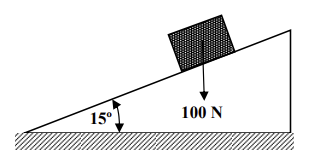
\includegraphics[width=0.5\columnwidth]{GATE/2016/XE/figs/ass3_d_q3.png}
    \caption{}
    \label{fig:placeholder-xeq3}
\end{figure}
\item A block $A$ on a smooth inclined plane is connected to block $B$ as shown in the figure using an inextensible cord which passes over a mass-less and friction-less pulley. Initially, the block $B$ is constrained to be at rest. If the constraint on block $B$ is released, the magnitude of velocity (in m/s) of the block $B$ after $2$ seconds from its release is \rule{1cm}{0.01pt}. (assume $g=10 \ \text{m/s}^2$).
\hfill(XE 2016)
\begin{figure}[H]
    \centering
    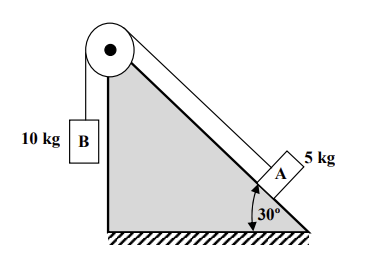
\includegraphics[width=0.5\columnwidth]{GATE/2016/XE/figs/ass3_d_q11.png}
    \caption{}
    \label{fig:placeholder-xeq11}
\end{figure}



